\documentclass{article}
\usepackage{geometry,tikz}
\usetikzlibrary{arrows,decorations.markings,calc,fit}
\geometry{paperwidth=18.5cm,paperheight=6.8cm,left=2pt,right=2pt,top=2pt,bottom=2pt}
\pagestyle{empty}
\setlength{\parindent}{0pt}
\tikzset{%
object/.style={draw,font=\tt},
objects/.style={font=\tt, nodes={anchor=base}},
create/.style={draw,-o},
filled/.style={draw,-*},
contains/.style={draw,-(,dashed},
createfill/.style={draw,decoration={markings,
                                    mark= at position -6.5pt with {
                                                      \fill[white,draw=black](0,0)   circle(2.5pt);
                                                      \fill[black]           (4.5pt,0) circle(2.5pt);
                                                                }
                                   },
                                   postaction={decorate}},
derive/.style={stealth-},
parameter/.style={font=\footnotesize, fill=white, inner sep=1pt, outer sep=0pt, opacity=0.8, text opacity=1, rounded corners},
limit/.style={dashed, very thick, gray}
}
\pgfdeclarelayer{background}
\pgfdeclarelayer{backbackground}
\pgfsetlayers{backbackground,background,main}
\begin{document}
\centering
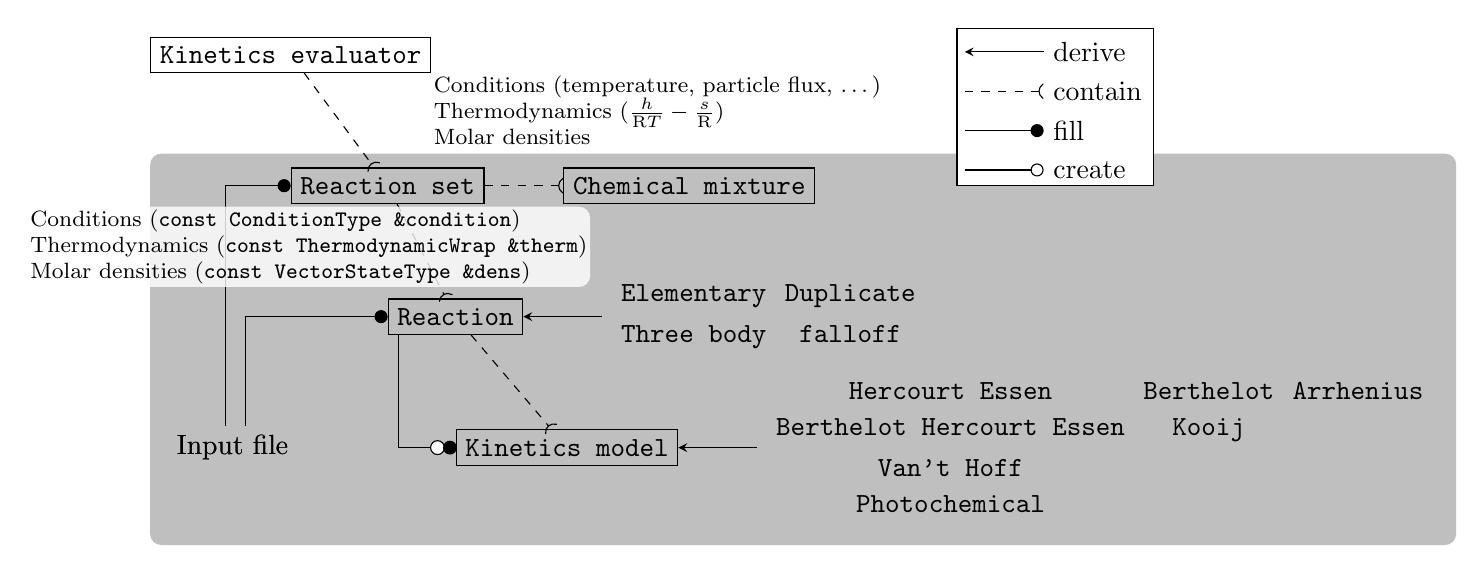
\begin{tikzpicture}
\node[object]                (kinmol)   at (0,0)                {Kinetics model};
\node[object,above = 1.2cm]  (reac)     at (kinmol.north west)  {Reaction};
\node[object,above = 1.2cm]  (reacset)  at (reac.north west)    {Reaction set};
\node[object,above = 1.2cm]  (kineval)  at (reacset.north west) {Kinetics evaluator};
\node[object,right = 1.0cm]  (chemix)   at (reacset.east)       {Chemical mixture};
\matrix[objects,right = 1cm 
             ,align=left]    (chemproc) at (reac.east)          {\node{Elementary}; & \node{Duplicate};\\
                                                                 \node{Three body}; & \node{falloff};\\};
\matrix[objects,right = 1cm 
             ,align=left]    (kinmod)   at (kinmol.east)        {\node{Hercourt Essen}; & \node{Berthelot}; & \node{Arrhenius};\\
                                                                 \node{Berthelot Hercourt Essen};            & \node{Kooij};\\
                                                                 \node{Van't Hoff}; \\ 
                                                                 \node{Photochemical};\\};
\node[parameter,below right,
        align=left]          (parKE.south east)    
                                        at (kineval.south east) {Conditions      (temperature, particle flux, \dots)\\
                                                                 Thermodynamics  ($\frac{h}{\mathrm{R}T} - \frac{s}{\mathrm{R}}$)\\
                                                                 Molar densities};
\node[parameter,below = 1pt,
        align=left]          (parRS)    at ([xshift=-1cm]reacset.south)      {Conditions      (\verb!const ConditionType &condition!)\\
                                                                 Thermodynamics  (\verb!const ThermodynamicWrap &therm!) \\
                                                                 Molar densities (\verb!const VectorStateType &dens!)};

\begin{pgfonlayer}{background}

\foreach \m/\c in {reac/chemproc,
                   kinmol/kinmod}
{
  \draw[derive] (\m) -- (\c);
}
\node[left=2cm]  (file) at (kinmol.west)   {Input file};
\foreach \m/\c in {kineval/reacset,
                   reacset/reac,
                   reacset/chemix,
                   reac/kinmol}
{
  \draw[contains] (\m) -- (\c);
}
\node[left=2cm]  (file) at (kinmol.west)   {Input file};

\foreach \o/\xs in {reac/10,reacset/-10}
  \draw[filled] ([xshift=\xs mm]file) |- (\o);

\foreach \f/\o in {reac/kinmol}
  \draw[createfill] ([xshift=4pt]\f.south west) |- (\o.west);
\end{pgfonlayer}


\draw[fill=white] ([xshift=6cm]reacset.east)coordinate (leg) rectangle +(2.5,2);

\draw[create]   ([yshift=2mm,xshift=1mm]leg) -- ++(1,0)node[right]{create};
\draw[filled]   ([yshift=7mm,xshift=1mm]leg) -- ++(1,0)node[right]{fill};
\draw[contains] ([yshift=1.2cm,xshift=1mm]leg) -- ++(1,0)node[right]{contain};
\draw[derive]   ([yshift=1.7cm,xshift=1mm]leg) -- ++(1,0)node[right]{derive};

\begin{pgfonlayer}{backbackground}
\fill[gray!50, rounded corners] ([yshift=5pt]reacset.north -| kineval.west) -|  ([xshift=5pt,yshift=-5pt]kinmod.south east) -| ([yshift=5pt]reacset.south -| kineval.west) -- cycle;
\end{pgfonlayer}
\end{tikzpicture}
\end{document}
